%Proposal Dissertation: Health inequalities in the retired population
% Project 1: Household Pension income and the sex differences in mortality

%------------------------------------------------------%
\documentclass[a4paper,10pt,oneside,english]{article}
%------------------------------------------------------%

\usepackage[left=2cm,top=2cm,right=2cm,bottom=2cm]{geometry}
%LANGUAGE
\usepackage[english]{babel}
\selectlanguage{english}

\usepackage{paralist}

%GRAPHIC SETTINGS
\usepackage{graphicx}
\graphicspath{C:/Users/y4956294S/Documents/Barcelona_CED_PhD/Proposal_PhD}
\usepackage[pdftex,colorlinks,a4paper,bookmarks=true,bookmarksnumbered=true,linkcolor=blue,citecolor=blue,urlcolor=blue]{hyperref}
\usepackage{wrapfig}
% for floats of graphs
\usepackage{float}
\usepackage{color}
% for the euro sign
\usepackage{eurosym}

%MATH-AND FORMULAR PACKAGES
\usepackage{amssymb}
\usepackage{amsmath}
\usepackage{mathtools}

%FORMATTING & FONT
% For formatting titles of appendices
\usepackage{appendix}
% for bold writting
\usepackage{bm}
\usepackage{dsfont}
\usepackage{lscape}
\usepackage{listings}
\usepackage{tabularx}
\usepackage{ragged2e}
\usepackage{setspace}
\usepackage{framed}
% for graphs and tables
\usepackage{caption}
\usepackage{palatino,url}
% For footnotes and author affiliation
\usepackage{authblk}

%LITERATURE
\usepackage[square,numbers,sort&compress]{natbib}
\renewcommand{\bibsection}{}
\usepackage{booktabs} % To thicken table lines
\usepackage{hyperref}
% Translates Input (formulars) into latex
%\usepackage{inputenc}
% -----------------------------------------------------------------------------% 

	% Front Page %
	%------------%

\title{\begin{center}
		\sffamily
		\large {IUSSP International Population Conference 2017}\\
		\Large{Health and Mortality during the transition to retirement in Spain}\\
		\large{Analysis of Mortality Differences by Social Position in Spain with the Longitudinal Population Register of Andalusia (BDLPA)}
\end{center}}
\author[1]{Mathias Voigt}
\author[3]{Fransico Viciana} 
\author[2]{Diego Ramiro}
\author[3]{Rosa C\'{a}novas}
\author[3]{ V\'{i}ctor Monta\~{n}\'{e}s Cobo}
\affil[1]{Center for Humanities and Social Sciences, Spanish National Research Council \& Universitat Aut\`{o}noma de Barcelona}
\affil[2]{Center for Humanities and Social Sciences, Spanish National Research Council }
\affil[3]{Institute for Statistics and Cartography in Andalusia}

\renewcommand{\baselinestretch}{1.5}

\begin{document}
	\date{}
	\sffamily
	\maketitle
	
                           %% Short Abstract %%
\begin{abstract}
	\noindent
	\textbf{Background:} After decades of exceptional mortality improvements paired with low fertility South European societies have to face the challenges of heavy population aging. Especially the prospect of large baby boomer cohorts approaching retirement age raises concerns about the sustainability of social security and pension funds. For the adjustment and reformation of pension systems, it will be essential to address the socioeconomic health gradient and mechanism behind structural inequalities in the retired population. In particular with regard to aspects of social fairness, the quantification of existing inequalities in health and mortality within the retired population can contribute to the anticipation of prospective effects on the population health.\\
 	\textbf{Method:} We analyze the impact of several socioeconomic and demographic indicators on mortality during the transition to retirement by applying stratified Cox Proportional Hazard regression models. This analysis is conducted, using the \emph{"Base de Datos Longitudinal de Poblaci\'{o}n de Andaluc\'{i}a"} (BDLPA), a register-based individual level data base which is linked to the Andalusian social security data set NIS for the years 2011 to 2015.\\
 	\textbf{Results:} While the results for the male population indicated the existence of a socioeconomic mortality gradient, the analysis could not confirm a similar effect for Andalusian women. Only the group with the lowest household income seemed to be affected.\\
 	\textbf{Conclusion:} Although there is no indication for a clear socioeconomic gradient, the analysis of Andalusia's retired population confirmed the increased mortality risk of the group at the bottom of the income distribution.
					% What is missing? %
					%% - exact research question = What is the Big E and small e's?
					%% - What methods you want to use?
					%% - Abstract needs to become the structure of the paper (!)
				    %% Flexible parametric models apply cubic splines to fit a baseline failure rate in a survival process and have advantageous properties compared to the widely used Cox PH model
\end{abstract}
\newpage
%
%%% What needs to be done?
%\section*{The project - plan and general ideas}
%{\large Big E - empirical question that I try to answer}\\
%\textbf{How does the social position (education \& income) determine health during the transition to retirement?}\\
%We aim to examine the effects of pension income and eligibility age (both under jeopardy through latest pension reforms) on health and mortality in Andalusia from 2011-15. We argue that pension size and eligibility age could affect mortality during the transition to retirement (direct income hypothesis) regardless the social status (measured through education, car ownership, and housing regime). While we expect these effects to be much stronger for men, we are looking for a way to find indicators for female survival after retirement. - In forms of questions and assist question: 
%	\begin{enumerate}
%		\item Why can we not find mortality differences by socio-economic position for women (Are women more equal?) - with similar working histories - would there mortality be different?
%		\item How is reaching retirement age in good health determined by social position?
%		\item How does the option for early retirement affects longevity (Thomas idea)? + Does the "income cut" through entry in retirement has an impact?
%	\end{enumerate} 
%\subsection{To do! -  the story line}
%\begin{enumerate}
%	\item Population aging is a heavy burden for the Spanish household - which used to be stable and almost debt free - and especially since the crisis hit, politicians started to postpone pension eligibility ages and pension sizes (social security reform)
%	\item the claim a fair formula which is based on average life expectancy = since we can expect heterogeneity with regard to mortality rates by socioeconomic status (basically the existence of a social mortality gradient), it can be assumed that the burden is not shared equally
%	\item To confirm our assumption it is necessary to know to what extent the pension size and the eligibility age affects mortality of pensioners regardless of other social indicators like education
%	\item Since we expect differences in the average pension size, educational attainment for men and women (female life courses in these generations of Andalusians generally differ from the classic male life course in terms of educational attainment and labor market history), a separate analysis will be necessary = as we know from the EPC 2014 there will be significant effects for men but ambiguous ones for women
%	\item We have a way to analyze the effect of the partners income for married couples who lived together in 2001, did not get divorced until 2011 and retired in the course of time = it needs to be examined what the share of these people is and if they are by any mean representable
%\end{enumerate}
%\subsection{To consider!} 
%\begin{itemize}
%	\item the Spanish social security/health system is modern, very efficient and relatively easy to access (until changes in 2012 - paper) 
%	\item Why should there be differences in health/mortality? (Braveman et al. 2009 paper)
%	\begin{enumerate}
%		\item mortality difference are a mixture of behavior, access, environment, social position, genetic predisposition (which should not be affecting our analysis)
%		\item accumulated disadvantages of individuals in economically and socially disadvantaged milieus (behavioral)
%		\item changes in health care = 2012 reform; period effects of the economy crisis
%	\end{enumerate} 
%	\item \textbf{Define the study population!} = everybody who paid into social security and is retiring within the study period or before (left truncation?) + are in the census of 2001 and in the social security data of 2011-2015
%	\item there is a good descriptive overview on old-age poverty in M.Oris et al. (2017) paper (Long Lives and Old Age Poverty) = three major phases in developed European countries
%	\item proof assumptions about life course trajectories and forms of living in old age in Andalusia
%	\item account for different definitions of retirement including partial retirement - Fisher article! - consider to look for differences between "early", "on-time" and "late" retirement
%	\item Remember to frame the transition to retirement; it is dependent on the life and working life course of an individual (see Elder 1994) = life course perspective emphasize the role of contextual embeddedness, interdependency of life spheres, timing of life events and human agency (Fisher et al. 2016)
%	\item retirement is a stressful life event leading to a substantial loss of social network connections and is often associated with cognitive and physical decline
%\end{itemize}
%\newpage
% ----------------------------------------------------------------------------------------------------%
% Background section %
% 1. Short (1 Paragraph) about development of life expectancy in general and in Spain
% 2. Why could this be a problem (ODR) and what is the solution (Pacto de Toledo) -  Explain in 1-2 paragraphs (demographic momentum)
% 3. Why is it problematic using the general life expectancy (heterogeneity is not covered) & leading to the research: What do we need to know? (What structural distortions exist and who would be affected)
 %% It is probably good idea to mention the relationship between income and health at this point
 %% Here we can also fit the idea: If wealthy people live longer, we have to pay higher pensions for a longer time + it is unfair towards the low paid contributers to raise the entry age (or not because they are getting healthier)
% Since this study will be conducted with Spanish (Andalusian) data, (and also since we know what we will find for men and women) it makes sense to write 1. paragraph about the mortality differences and 1 paragraph about the labor market situation
% ----------------------------------------------------------------------------------------------------%
% ----------------------------------------------------------------------------------------------------%
% That is why I originally thought, that I could create "story" around the population which is going to retire - that go through major life changes, change their exercising and drinking habits and most importantly experience a reduction of their income. The biggest argument in this case would be from a life course perspective, that low pension size and little contribution years would be a proxy for a fragmented working life and indicate a cumulative disadvantage in the sense that somebody who had no job in the past, had less chances for self fulfillment and access to many things that make life better like going on vacations (indirect income hypothesis). This person will also have a lower pension and a life long disadvantage relative to "wealthier" individuals might pay off through a higher mortality. So far the story, but it is difficult to test because of all the "background noise".
% ----------------------------------------------------------------------------------------------------%
\sffamily
\section*{\textsf{Introduction}}
South Europe experiences a rapid change of their population structure. Decades of low birth rates in combination with a historically unique improvement in mortality rates across all ages have led to shrinking and heavily aging populations \citep{RN19,RN69}. Despite the remarkable opportunity for millions of people to enjoy longer lives in a better health compared to previous generations \cite{christensen2009ageing,RN14}, the growth of average human life lengths entails considerable challenges for social security systems \citep{RN68}. A growing number of welfare or pension recipients is increasing the pressure on the working age population which itself is declining at the same time. The Old-Age Dependency Ratio \footnote{\textsf{$D=\frac{N_{65+}}{N_{15-64}}$; where $N_{65+}$ is the population 65 years and older, and $N_{15-64}$ the population in working ages}} in Spain and Italy is projected to increase from 0.33 to about 0.5 until 2050 and therewith exceeds values of most North and Central European countries \citep{RN9,RN34}.\\ % Financial crisis = Demographic crisis scenario
Besides the pressure caused by demographic aging, South European economies were hit extraordinarily hard by the global financial crisis in 2008. Austerity policies in answer to the recession additionally jeopardized the sustainability of social service budget and public pension funds \cite{RN64,RN141}. Consequently, policy makers were forced to react and initiated modifications with regard to the access to public pensions following the example of other European countries. In Italy and Spain adjustable conversion factors were implemented in the pension formula which determine future pension sizes and eligibility ages based on life expectancy \cite{Sanchez2014,de2014altered}. The extension of the working life in particular promises to be a relative efficient and cost-effective adjustment to the population development and would postpone shortages of pension funds to the future \citep{RN61,RN65}.\\ % What they change might not affect everybody to the same extent
Regarding social fairness, however, it is important to ask if the additional burden which is imposed on the population by prolonging their working lives and cutting their pensions is shared equally. In other words, will such reforms affect particular social groups more negatively than other and increase existing health inequities? Since the average life expectancy was chosen to determine the eligibility to full pension, heterogeneity with regard to survival remains unconsidered. Thus, if structural inequalities with regard to health and survival exist within the society and are related to forms of occupation or other socioeconomic characteristics, raising the eligibility age could manifest and reinforce advantages of social groups over others.\\
In order to estimate the impact of changes in the eligibility age and pension size on the health and survival, it is necessary to acquire more detailed knowledge about the structural mechanisms which shape the health of the retiring population. Apart from the aspect of fairness, knowledge about structural health differentials by socio-economic and demographic characteristics are essential for the estimation of expenditures for future care need. We aim to fill a part of this void with our analysis of structural mortality differences during and after the transition to retirement. After describing the underlying mechanisms for our examination, we introduce a relatively underused longitudinal data structure provided by our project partner, the Institute for Cartography and Statistics of Andalusia (ICEA). The register-based data infrastructure allowed us to obtain follow-up data for mortality after entry into the public pension system in combination with the Spanish Population and Household census of 2001. We apply stratified Cox proportional hazard models to separately estimate the mortality differentials for women, men and married couples depending on various socioeconomic measures over time. 
%%% ---- Results ---- %%%


%%% --------------------------------------------------------------------------------------- %%%
%%% Here sits the soul of the article!  %%%
%%% What is it all about? What is the contribution to the field?
%%% 
  % Analysing health/mortality differences in the retiring population - dependent on their entry age and pension size, education and a bunch of other mediating variables
  % age at death is the outcome variable
  % We separately analyze men and womens status - biological and behavioral differences in LE make it difficult to compare the two groups (at eligibility age they have different mortality risks)
%%% --------------------------------------------------------------------------------------- %%%
\section*{\textsf{Background}}
\subsection*{\textsf{Structural inequalities and health}}
% How is survival determined in modern, high income societies? %
In spite of the multitude of explanation for the historical mortality decline \citep{riley2001rising}, it is hard to imagine that average human life lengths will continue to increase at current rates if improvements of living standards, entitlement to full pension benefits, or access to advanced medical treatments are not shared equally. Although most modern, high income countries provide comprehensive and affordable health care for their citizens, there is evidence for survival differences depending on income, education and occupation type. Numerous researchers point out the existence of a mortality advantage for better educated and wealthier individuals over lower educated and less wealthy ones  \cite{RN214,RN26,RN28,RN29,mackenbach2008socioeconomic,RN70}. Whereas the impact of income on health is probably rather direct in developing country where it determines the access to fresh water and adequate nutrition, it is assumed to work through access to opportunities for social participation in more developed countries \cite{RN35,RN39,RN41}. One of the two major hypothesis explaining the impact of income on health is the Absolute Income Hypothesis (AIH). It assumes an indirect relationship between personal income and average health. The Relative Income Hypotheses (RIH) based on Rogers (1979) \cite{rodgers1979income}, in contrast, relates the average population health level to the income distribution on a society level \citep{RN2}.\\
% Growing income inequalities on a macro-level - Reinforcement of the educational gradient %
An economic and education gradient with respect to survival and health needs to be considered for the adjustments of pension reforms on the basis of average life expectancy, especially in times of growing income inequalities in many OECD countries \cite{RN74,corak2013income,RN47}. Increasing the eligibility age and taking away possibilities for early retirement can possibly have very different effects on the longevity of social groups and in return increase the costs through higher care need. Nevertheless, the relationship between socio-economic characteristics is controversial and strongly depends on measurement strategies. The use of cross-sectional information will make it for example hard to distinguish if individual health problems determine the income instead of the other way round. Moreover, aggregated income measures cannot be consistently linked to individual-level health unless the relationship is linear \citep[cf.][]{RN49}. In our contribution, we account for these limitations by applying a unique data infrastructure which allows us to examine the link between individual level pension income and mortality in Andalusia, the second biggest and most populated of the 17 Spanish autonomous communities \citep{RN113}.\\
Since retirement pensions are closely related to the individual life time social security deposits and therewith the working life course trajectories, there are substantial differences in the response to pension measures between men and women. In the context of Spain and Andalusia gender inequality in paid labor as well as other social spheres is historically relatively high and has only recently been addressed at a broad political level \citep{guner2014gender}. With regard to the cohorts under observation, variations and distributions in life time earnings, educational degrees and accumulated pension income through a constant employment are extensive between the male and the female population \citep{gonzalez2014gender}. Moreover, differentials in biological predispositions and risk related behavior have also let to relatively big gender gap in mortality in Spain and other South European countries \citep{caselli2010increasing,gjoncca2005sex,cockerham2005health}. Currently the female advantage measured in years of life expectancy at birth is 5.52 years Spain (2014) and 4.73 years in Italy (2012) \footnote{Calculations based on data downloaded from the Human Mortality Database, University of California, Berkeley (USA), and Max Planck Institute for Demographic Research (Germany). Data downloaded on 26.01.2017 \citep{RN21}}. 

% -----------------------------------------------------------------------------------------------------%
\subsection*{\textsf{The transition to retirement and its association to ill health}}
% This will be the part when we move from the macro to the micro level perspective. While we first pointed out the possible overall problems of changing the eligibility age and the existence of groups with different "average" life expectancies, it is necessary to examine the transition to retirement from the individual perspective and as embedded in the life course. In the end we will also find an answer to the question to what extent these processes are interconnected - how can macrolevel decisions affect microlevel outcomes?
% Also mention - endogeneity problem (what comes first, retirement or health issues)
At an individual level, entering retirement is potentially stressful life course event which is associated with a substantial loss of social network resources and can be, dependent on the sociocultural context, perceived as entering a period of cognitive and physical decline \citep{RN205}. % that could be dangerous for your health %
Especially during the transition period, various spheres of life such as the daily activities, family relations and financial wellbeing are exposed to substantial changes \citep{RN209}. Given the increasing share of physiological frail individuals in these age groups \citep{RN204} and depending on the financial and family support network, such changes could trigger downward spirals in health and ultimately lead to fatal outcomes.\\ 
Regarding the associations between mortality and the transition to retirement, the results are mixed and indicate that we deal with a very dynamic process \citep{RN202, RN208, RN199, RN207, RN205}. While the meaning of retirement does not only change as social (age) norms evolve, requirements for entering and pension size are as well dependent on the economical and demographic development. Therefore, definitions for retirement are not static and vary along the three major dimensions timing, completeness and voluntariness \citep{RN203}. Furthermore, the decision to retire is highly individual, prone to sudden changes and stimulated by various life course events and push and pull factors. Arguably the biggest obstacle with regard to the association between worsening health and retirement is their endogenous relationship \citep{RN195}.\\
% -----------------------------------------------------------------------------------------------------%
% Risk factors - continuation theory + financial incentives + perception and social norms 
%%%% Next steps:
% ! Remember that the goal is to compare different socioeconomic groups and not examine the effect of retirement age or retirement on mortality
% 1. Point out why it does still make sense to look at the effects of social position during the transition to retirement. It is possible that the stress levels vary by socioeconomic postion and that early retirement options might be necessary for some groups but not others. ! In the end you will need a sentence or two that bring you back to the socioeconomic differences.
%%%% Mention the theories of accumulated disadvantages in combination with frailty theories
% -----------------------------------------------------------------------------------------------------%

% 2. Mention that life courses of men and women are different - especially for these generations of Andalusians. Also their average mortality risk around the entering to retirement as well as their response to aging is different and therefore it make sense to compare men to men and women to women
\subsection*{\textsf{Mortality differentials and social inequalities in South Spain}}
% "in the context of Andalusia" / "coming to age"
% --------------------------------------------------------------------------------------------------- %
% Why does it make sense to do the analysis here (in Andalusia)?
% It is the most deprived and aged region of Spain. It has major problems after the financial crisis...
%Considering objective aggregate measures, the Spanish population 

Although mortality differentials by socioeconomic characteristics seem to be rather moderate in South European countries in comparison to other European regions \citep{RN214}, their current demographic, social and economic development entails various potential challenges regarding regional and economic inequality.
%% Short the Spanish development : rapid increase in LE (because they came from lower levels) + low levels of disability - may be mentioning that the assumed advantage can be reduced to two major diseases related to smoking "equality" - everything else is not as good as they think
%% Andalusia as deprived rural area where nobody wants to live - outmigration and 
Studies on the onset of disabilities and age related chronic diseases reveal that these historical gains in average life span are generally spent in good health \citep{RN107}. Although the most recent economy crisis and the related reductions of the health and social service system budget were expected to slow down the remarkable mortality improvements \citep{RN116,RN141}, short-term effects on overall survival even pointed towards a faster reduction of Spanish mortality rates. Whereas some studies found an elevated risks for suicide and mental health issues which correlate with the economic downward trends and increasing unemployment \citep{RN180,RN176}, mortality from most causes decreased after 2008 \citep{RN182}.
% ----------------------------------------------------------------------------------------------------%
While Spain's population , the transition to a regime with low fertility and mortality rates was remarkably rapid. 1941, two years after the end of the Spanish civil war, marks the beginning of the exceptional growth period with an increase in average life expectancy at birth for both sexes combined by more than ten years within four years (47.19 years - 57.79 years) \footnote{The series of Spanish life tables was downloaded from the Human Mortality Data Base (access date 01.08.2017) \cite{RN21}}. Following a short period of stagnation, a more moderate but long-lasting increase in life expectancy sets on in the 1950, probably related to the economic stabilization through (!!!). Since then, the period life expectancy at birth grew with except of a socio-political re-orientation period after the end of the dictatorship in the early 1970s, and arrived to be the European record for women during the last three consecutive years \citep{RN114,RN105}. 
% ----------------------------------------------------------------------------------------------------%
% connection to the regional level %
Our analysis is centered around Andalusia, which is the southern most and with about 8.3 million inhabitants (2016) most populated of the 17 Spanish autonomous communities \citep{RN113}. 
%% One sentence about the historical mortality disadvantages and economic problems of today
Although the predominantly rural region has experienced economic bottlenecks and strong selective outmigration of young healthy individuals throughout the twentieth century, in recent decades, not only economic and social indicators approximated the Spanish average but also Andalusian mortality rates. Analyses of small area differences have indicated that currently only a group of municipalities in the south west of the community is exposed to higher mortality rates than the Spanish average \citep{RN100}. While survival disadvantages were historically attributed to strong excess mortality of children and young adults, since the 1960, differences are contributed by the population older than 65 years \citep{RN105}.
%% heavily affected by the economy crisis!
With its historically rather instable economy, Andalusia was hit extraordinarily hard by the recent financial crisis which led to extreme job loss and a constantly increasing at-risk-of-poverty rate which reached with 35.4\% in 2016 far higher levels than the Spanish national average (22.2\%) \citep{RN184}. Since it can be assumed that the effects of a recession on mortality and health are somewhat time lagged, it is not surprising to find ambiguous short-term results for this relationship. The only exception is the sharp increase in mental health problems which is for example expressed through the vast increase in suicide attempts since 2008 \citep{RN136}.
%%% --------------------------------------------------------------------------------------------- %%%
%\subsection*{\textsf{Disparities in male and female life courses}}
%%% Gender differences in mortality as well as in labour force participation will be important to mention - the give you a good basis for a separate analysis of mortality
%Currently the female advantage measured in years of life expectancy at birth is 5.52 years Spain (2014) and 4.73 years in Italy (2012) \footnote{Calculations based on data downloaded from the Human Mortality Database, University of California, Berkeley (USA), and Max Planck Institute for Demographic Research (Germany). Data downloaded on 26.01.2017 \citep{RN21}}.
%\begin{itemize}
%	\item convergence and divergence of a gender gap in life expectancy throughout the last century (Mesle and Caselli)
%	\item life style and behavioral differences probably the main reason for a gap greater than 2-3 years
%	\item everything else can be assigned to biological differences (?)
%	\item due to these mortality differences it makes sense to separate males and females in an analysis of a particular time window centered around a transition related to age
%\end{itemize}

% Marriage statistics - especially to back the analysis up: How persistent are relationships/marriages?

%%%%%% For the assist questions! It makes sense to mention the different life course histories of men and women - especially these generations. Knowing the preliminary results, it will be necessary to explain beforehand why we might expect no large differences for women (low case numbers of women with complete working life history). - there has to be a better argument!


% ----------------------------------------------------------------------------------------------------%
% Goals - What is the research strategy of this paper? %
%% Explain in short (1-2 paragraphs) the what we are going to add to the discussion %%
%% 1. We will look at all cause mortality at the ages around retirement age %%
%% 2. We will have unique individual level data including pension size and type - observing cohorts which retire between 2011 and 2015%%
% Plan: Apply disparity measures to the population(graph shows opening and indicates more equality for women) - Repeat with Individual level data from Andalusia
% ----------------------------------------------------------------------------------------------------%
\section*{\textsf{Methodology \& Data}}
 % detailed individual level analysis with high quality data
 % life course perspective on a highly difficult subject matter - decision to retire often not voluntary
 % Quantify the differences in average survival for different social groups and see the impact of entering to retirement (see paper about Britian)
%\begin{itemize}
%	\item analysis of the effect of social position on survival/mortality after the transition to retirement
%	\item how does the entry age (by healthy and unhealthy subpopulations) and the pension size matter in the context = moderating effects? -  occupational history
%	\item Do individuals have a higher risk of dying dependent on their socioeconomic position?
%	\item Is it possible to estimate the average survival time of sub-groups??
%\end{itemize}
% ----------------------------------------------------------------------------------------------------%
% Data - Section on Andalusian data %
% ----------------------------------------------------------------------------------------------------%
%% More information about the background of the database = Why did they have the initiaitive? %%
	% register based time-to-event data for the Andalusian officially registered population
	% paired with the social-security data from 2011 to 2015 - which give us information about everybody who contributed to social security and 
Following an initiative of the Andalusian government in 1996, the Institute of Statistics and Cartography of Andalusia produced a register based longitudinal population dataset, the \textit{Base de Datos Longitudinal de Poblaci\'{o}n de Andaluc\'{i}a} (BDLPA). This relatively recently developed statistical infrastructure allows us to follow up death and out migration for an almost full sample of a synthetic cohort of the Andalusian population in 2001 to currently 2015. Based on the Spanish population and housing census of 2001 a major advantage of the data structure is the possibility to jointly apply it with other administrative population based data basis in Andalusia or Spain \citep{RN8}. For the examination of a possible socioeconomic gradient during and after the transition to retirement, we applied for the pension spell data set of the Spanish National Institute for Social Security (NISS) \citep{RN8b} and successfully linked information on the spells of retirement, widowhood and disability pensions for the years between 2011 and 2015 to the individuals in the BDLPA. While we have no detailed information on private pension schemes, the NISS provides data on the about 93\% of the population who receive a public pension \citep{RN215}.
% Since the data is gained through a administrative process, we had to exclude a number of incoherences. 
For the analyzes of health inequalities during the transition to retirement we focus on individuals in three states. Apart from the absorbing state death, which is our variable of interest, we observe everybody who has entered the public pension system between 2011 and 2015. Consequently, individuals in our study population can either still be employed or on the job market or they are retired. We assume that individuals are not able to change their state from retired to working. In order to capture earlier entries to retirement as well as have a reasonable cut of point we decided to observe only persons of age 55 or older at begin of the study in 2011. The legal eligibility age for early retirement was set to 61 by a royal decree in 2002 \citep{RN217}. Since there are occupational groups like workers in the mining industry who have separate benefit systems, we set the entry age to 55. We do not observe the mortality or the pension information for individuals older than 90 to avoid possible biases through missing data and errors. Since the data has been gained through administrative processes, in the transmission and linking process a number incoherences have occurred. We decided to take precautionary measures and exclude the age groups where possible data errors could have a large effect on the outcomes as consequence of small group size.\\
From the administrative raw data we generate two distinct data sets to examine socioeconomic differences by individual and household measures. The properties and distributions of important covariates are displayed in table 1. The data set with individual retirement spells contains information about 641.223 persons who received a public pension between 2011 and 2015 and have resided in Andalusia since 2002. Accounting for gender differences in life course trajectories, earnings, and mortality, we conduct a second analysis applying a subset of the full dataset which contains information on married couples who have received a public retirement pension. Regarding the data structure, the examination of married couples was the only possibility to extract information on the household income for our subsequent analysis of female mortality.
%\subsection*{\textsf{Variables}}
With regard to our focus on the impact of socio-economic position on health, the pension as well as the pension household income serves as our main explanatory variable. For easier access we collapse the continuous variables in four categories based on the income distribution of the population at risk.We further refined the socio-economic position of an individual by the highest obtained education degree, the contribution time to social security as proxy for a stable or fragmented working life, the ownership status of the home, and the access to personal motor vehicles. Age, sex and the household size at baseline enter the analysis as demographic variables. The second data set regarding the married couples additional contains information on age differences between the partners as well as the education and pension information of the partner. 

%% --------------------------------------------------------------------------------- %%
%% Cox model description
%% --------------------------------------------------------------------------------- %%
\subsection*{\textsf{Statistical Model}}
%% --------------------------------------------------------------------------------- %%
%% 1. Describe the models (Cox-Proportional Hazard Model) %%
%% 2. Describe the strategy = single steps of the survival analysis    %%
%% 2.1. Develop the model with the 7-step programm of Hosmer et al. 2011 %%
%% 2.2. Lifespan disparity measures %%
%% --------------------------------------------------------------------------------- %%

The most often used regression approach to survival data is unarguably the semi-parametric Cox Proportional Hazards Model \citep{mills2011introducing}. It is statistically robust and can be obtained for a wide range of data situations without specifying a underlying baseline distribution. The effect of the covariates on the individual hazard in the Cox model enters multiplicative as shown in equation 1 \citep{kleinbaum2010survival}.
\begin{equation}
h(t_j)=h_0 (t) \exp(x_j,\beta)
\end{equation}
where $h_0(t)$ represents the underlying baseline hazard function at time t and $\exp(x_{j,ß\beta})$ is the non-negative function of covariates. The model estimates are obtained through the maximization of a partial log likelihood function, a method which was as well developed by David R. Cox \citep{allison2014event}. He proposed to maximize just the right handed side of the formula with respect to βx, setting the derivate equal to zero and solving the unknown parameter \citep{Hosmer2011}. The unspecified baseline hazard from the left part of the formula is simply discarded for the further estimations which explain the word “partial” in the name of the method. The partial likelihood function is treated as an ordinary likelihood function but the maximization process has to be done through a numerical optimization method.
The decision to leave the baseline hazard unspecified allows users to avoid assumptions about the survival time distribution \citep{mills2011introducing}. Furthermore, it results in a statistically relatively robust model which is easy to apply, very effective in the stratified analysis of nuisance variables and allows for an easy adjustment for time periods when no individual is at risk \citep{allison2010survival,therneau2000cox}. Given the structure of the data sets we use for the analysis of socioeconomic differences on mortality, we had to allow our model to account for left truncation  \citep{cain2011bias}. For everybody who has entered the observation period as a pension recipient, the time under risk before the start date of the study remains unobserved. To account for the different baseline mortality risk and more important the working life trajectories of men and women separate models were estimated for the male and female population.


%% Describe the data as good as possible
%In spite of all popularity, the widely used Cox Proportional Hazards (PH) model implies some more or less problematic assumptions, most prominently, the theoretical constraint that the instantaneous risks of groups have to be proportional over time or the silent assumption that all individuals are homogeneous with regard to the experience of the event \cite{RN90}. To avoid these implications we apply a relatively rarely used survival model with advantageous statistical properties. The flexible parametric proportional hazards model, based on the work of Royston and Parmar (2002) \citep{RN93}, uses a restricted cubic splines to model the baseline failure rate and estimate arbitrary parameters. In contrast to the Cox PH model, the properties of this type of models allow to model complex time-dependent effects without manipulation of the data. Furthermore, these models provide the possibility to estimate absolute and relative effects as well as the incorporation of expected mortality and relative survival. The key advantage, however, is the availability of transformations for the parameters which allow group comparisons without assuming proportionality \cite{RN91,RN92}. The flexible parametric model can be introduced using the Weibull survival distribution \footnote{Assuming T $\thicksim$ Weibull $(\lambda,p)$ the survival and hazard function can be expressed as $S(t)=\exp (-\lambda t^{p}) \quad h(t)=\lambda pt^{p-1}$ where p is the defined as the shape parameter.}. Royston and Parmar suggest to use a link function $g\left[S(t;z)\right]$ which relates to the survival function $S(t;z)$ in the following way.
%	\begin{equation}
%	g\left[S(t;z)\right] = \ln\left[-\ln S(t;z)\right] = s(x;\gamma)
%	\end{equation}  % Explain the knots! %
%They choose $s(x;\gamma)$ to be a restricted cubic spline function with $x = \log(t)$ and $K$ knots. Such a spline function can fit almost any relationship between variables by creating $K-1$ derived variables. The model complexity is only governed by the number of knots, which are the break or boundary points where two polynomials are connected with each other \cite{RN97}.\\
%To proceed with estimation, $g[S(t;z)]$ is constraint to be monotonic at the extreme points. Since natural cubic splines are piecewise cubic polynomials with continuous first and second derivatives at the knots, by definition they guarantee monotonicity for reasonable large data sets. For the meaningful comparisons of survival risks by groups we estimate the logarithm of the cumulative hazard function, $\ln H(t;z)$. The cumulative log hazard is is another way to express $g[S(t;z)]$ \footnote{$\quad ln{H(t)}=g[S(t;z)]=ln[-ln{S(t)}]$} and has the advantage of incorporating covariates as linear effect of log time. The log cumulative baseline hazard of the flexible proportional hazards model can be easily related to the spline function $s(x;\gamma)$. Since $ln{H_0(t)}=ln[-ln{S(t)}]$ the fixed covariate vector \textbf{z} adds linearly as shown in the equation 2.
%	\begin{equation}
%	\ln H(t;z)=\ln H_0(t)+\beta^{T}z = s(x;\gamma)+\beta^{T}z
%	\end{equation}
%In contrast to the Cox model, we estimate the full maximum likelihood function for this model type as shown for the case of a log cumulative hazard function in equation 3. Let $\eta = s(x;y)+\beta^{T}z$. The likelihood function can be expressed as follows.
%	\begin{equation}
%	l=\left\{\begin{matrix}
%	\frac{1}{t}\frac{ds(x;y)}{dx}\exp(\eta-\exp\eta)\\ 
%	\exp(-\exp \eta)
%	\end{matrix}\right.
%	\end{equation}
%The upper part of the equation is applied to uncensored observation and the lower for censored ones. Starting values for the optimization process can be obtained by graphic tests or the estimation of Cox PH model with the same covariate vector $z$. Standard errors of fitted values $\hat{\eta_{i}}$ are obtained by the observation matrix for $\hat{y}$ and $\hat{\beta}$ following the Maximum Likelihood Estimation whereas a bootstrap technique is applied for the confidence intervals for the hazard function.
%%% accessment test for the best model
%We use the \emph{flexsurvspline} command from the R package \emph{flexsurv} to fit the model. Besides the flexible parametric proportional hazards model the package also allows to fit flexible proportional odds or probit model \cite{RN94}. 

%\begin{itemize}
%		\item In theory we have a multi-state process with three possible states (working, retired, and death) = \textbf{Fran is not in favor of this one, because we will miss a lot of the unemployed}
%		\begin{itemize}
%			\item \textbf{Anyways:} There is a possibility to model multi-state survival data with the \textit{flexsurv}package = see Jackson (2016, p.20-28), and for the original idea Andersen and Keiding (2002)
%			\item That would be a possible idea for a follow-up analysis (! check what are the characteristics of the once who make it to retirement age)
%		\end{itemize}
%		\item there is the possibility to apply a Cox Proportional Hazards model with death as event and the only possibility for right censoring are the end of the study period or moving away from Andalusia
%		\item another option would be a flexible parametric model using cubic splines for the baseline hazard (see slides from Lambert) (\textbf{That is the choice for the main analysis!!!})
%		\item may be later = look at the general additive models
%	\end{itemize}	
\section*{\textsf{Results}}
All conducted models show mixed effects of the pension income on the relative risk of dying. In the analysis containing all individuals who have received a pension between 2011 and 2015, the most categories of the income variable show no statistically significant impact on the hazard (table 1). The exception are the men who receive a public pension between 1000 and 1999 Euro a month. Their risk of dying in comparison to the reference group of men who own more than 2000 Euro monthly is about 6\% increased. In the case of the female population, the hazard of dying does not significantly vary by their pension income. The results for education as inequality dimension are more prevalent. The men with a secondary or higher education are highly significant and lower risk of 4.7\% of dying compared to their less educated counterparts. The effect for women is with about 8.4\% sightly elevated. As a further socioeconomic impact factor for mortality, the ownership status of the house or apartment the persons lives in indicates a mortality advantage of the presumably wealthier individuals. There is also strong evidence that a lack of access to a car and therewith reduced mobility affects the relative risk of dying for both sexes. The effect size is with 1.224 about 12\% higher for men than for women compared to individuals who own one or more motor vehicles. Also a protective effect of marriage was prevalent in both populations.\\
The Cox proportional hazard model results based on the married population of 2011 where both partners have retired until 2015 and were left truncated are displayed in the table 2. The income variable relates to the pension income of a house with two retired individuals and behaves similarly to the individual income. In the case of the married couples, the group with a household income of less than 1000 Euro per month were estimated to have a highly significant increased risk of dying within the time period under observation. Notable, the hazard differs relatively strong between men and women. While women living in a household with a monthly income of less than 1000 Euro per month are exposed to a 73.5\% higher risk of dying compared to their counterparts who live in households with more than 2000 Euro per month, the relative risk of men in the lowest income category to die is almost 4 times higher than for their more wealthy counterparts. Once the education of the partner is considered the highest obtained degree does not seem to influence the hazard extensively. With regard to the retirement timing, in time and late entry to retirement seem to be related to a lower risk of dying. The effect sizes are possibly biased by the endogenous relationship between health problems and early retirement. In the analysis it was accounted for the reception of a disability support pension before entering retirement. Here certain requirements have to be fulfilled, hence a bias cannot be excluded.
% \begin{figure} [h]
% 	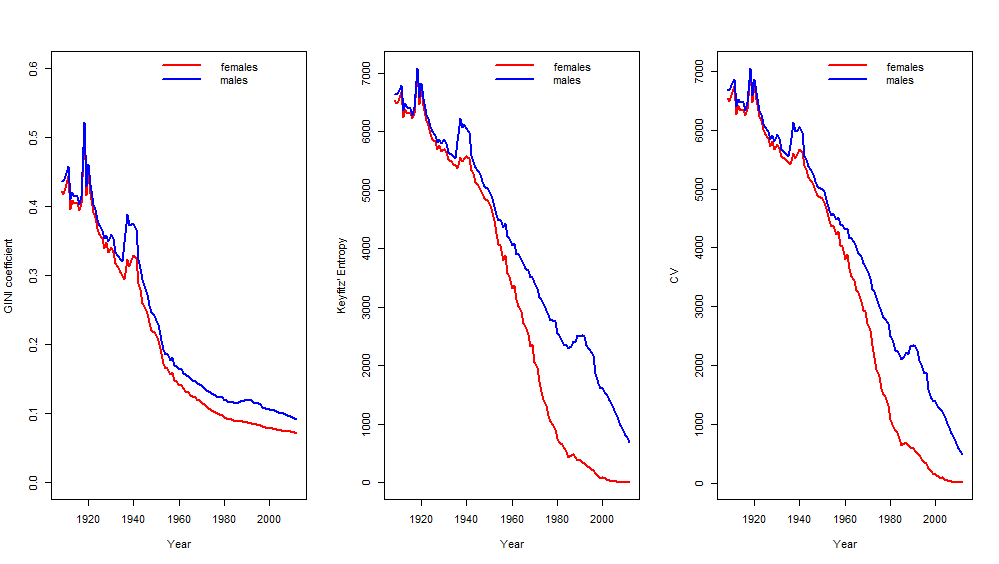
\includegraphics[scale=1, width=1 \textwidth]{lifespan_disparity_ESP}
% 	\caption{Lifespan disparity measures by sex. From the left: Gini-coefficient, Keyfitz\' entropy, Coefficient of Variation (own calculation)}
% \end{figure}

%\subsubsection{Descriptive Statistics}

% Table created by stargazer v.5.2 by Marek Hlavac, Harvard University. E-mail: hlavac at fas.harvard.edu
% Date and time: vi., sep. 29, 2017 - 15:23:51
\begin{table}[H] \centering 
	\caption{\textsf{Cox PH Model - Estimated hazard of dying for pension recipients between 2011-2015}}
	\label{} 
	\begin{tabular}{@{\extracolsep{5pt}}lrr} 
		\\[-1.8ex]\hline 
		\hline \\[-1.8ex] 
		& \multicolumn{2}{c}{\textit{Dependent variable:}} \\ 
		\cline{2-3} 
		\\[-1.8ex] & \multicolumn{2}{c}{Relative mortality risk} \\ 
		\\[-1.8ex] & males & females\\ 
		\hline \\[-1.8ex] 
		1000-1999  Eur/month & 1.059$^{**}$ (1.021, 1.097) & 1.076$^{}$ (0.923, 1.229) \\ 
		& & \\ 
		500-999 Eur/month & 1.035$_{.}$ (0.997, 1.073) & 1.036$^{}$ (0.884, 1.188) \\ 
		& & \\ 
		$<$ 500 Eur/month & 1.012$^{}$ (0.960, 1.064) & 1.004$^{}$ (0.849, 1.159) \\ 
		& & \\ 
		Secondary/Tertiary Ed. & 0.953$^{***}$ (0.932, 0.973) & 0.916$^{***}$ (0.871, 0.960) \\ 
		& & \\ 
		$<$ 20 y. contrib. & 1.055$^{**}$ (1.016, 1.093) & 1.015$^{}$ (0.979, 1.051) \\ 
		& & \\ 
		$>$ 40 y. contrib. & 0.939$^{***}$ (0.923, 0.955) & 1.025$^{}$ (0.959, 1.091) \\ 
		& & \\ 
		in time ret. & 0.851$^{***}$ (0.835, 0.868) & 0.834$^{***}$ (0.789, 0.879) \\ 
		& & \\ 
		late ret. & 0.800$^{***}$ (0.764, 0.836) & 0.812$^{***}$ (0.758, 0.866) \\ 
		& & \\ 
		birth year (cohort) & 1.007$^{*}$ (1.001, 1.012) & 1.023$^{***}$ (1.012, 1.033) \\ 
		& & \\ 
		married & 0.801$^{***}$ (0.770, 0.832) & 0.902$^{***}$ (0.857, 0.947) \\ 
		& & \\ 
		widowed & 0.905$^{***}$ (0.865, 0.946) & 0.979$^{}$ (0.934, 1.024) \\ 
		& & \\ 
		divorced & 1.089$^{**}$ (1.026, 1.153) & 1.007$^{}$ (0.894, 1.120) \\ 
		& & \\ 
		own house/apt. & 0.935$^{***}$ (0.899, 0.971) & 0.910$^{**}$ (0.843, 0.977) \\ 
		& & \\ 
		rent & 1.116$^{***}$ (1.068, 1.164) & 0.991$^{}$ (0.902, 1.080) \\ 
		& & \\ 
		no vehicles & 1.224$^{***}$ (1.207, 1.241) & 1.099$^{***}$ (1.066, 1.131) \\ 
		& & \\ 
		\hline \\[-1.8ex] 
		Observations & 441,329 & 199,894 \\ 
		R$^{2}$ & 0.005 & 0.001 \\ 
		Log Likelihood & $-$719,892.600 & $-$178,122.400 \\ 
		Wald Test (df = 17) & 2,081.840$^{***}$ & 239.440$^{***}$ \\ 
		LR Test (df = 17) & 2,014.293$^{***}$ & 234.433$^{***}$ \\ 
		Score (Logrank) Test (df = 17) & 2,091.617$^{***}$ & 239.909$^{***}$ \\ 
		\hline 
		\hline \\[-1.8ex] 
		\textit{Note:}  & \multicolumn{2}{r}{$^{*}$p$<$0.1; $^{**}$p$<$0.05; $^{***}$p$<$0.01} \\ 
	\end{tabular} 
\end{table} 
%
% ------------------------------------------------------------------------------------------------------ %
% ------------------------------------------------------------------------------------------------------ %
%
%% Couples and household income
% Table created by stargazer v.5.2 by Marek Hlavac, Harvard University. E-mail: hlavac at fas.harvard.edu
% Date and time: vi., sep. 29, 2017 - 16:26:46
\begin{table}[H] \centering 
	\caption{\textsf{Cox PH Model - Estimated hazard of dying for married pension recipients between 2011-2015}}
	\label{} 
	\begin{tabular}{@{\extracolsep{5pt}}lcc} 
		\\[-1.8ex]\hline 
		\hline \\[-1.8ex] 
		& \multicolumn{2}{c}{\textit{Dependent variable:}} \\ 
		\cline{2-3} 
		\\[-1.8ex] & \multicolumn{2}{c}{Relative mortality risk} \\ 
		\\[-1.8ex] & males & females \\ 
		\hline \\[-1.8ex] 
		1000-1499  Eur/month & 0.960$^{}$ (0.888, 1.032) & 0.989$^{}$ (0.839, 1.138) \\ 
		& & \\ 
		1500-1999  Eur/month & 0.962$^{}$ (0.877, 1.047) & 1.034$^{}$ (0.863, 1.205) \\ 
		& & \\ 
		$<$ 1000 Eur/month & 3.998$^{***}$ (3.914, 4.082) & 1.735$^{***}$ (1.539, 1.931) \\ 
		& & \\ 
		high education. & 1.014$^{}$ (0.947, 1.082) & 1.172$^{*}$ (1.026, 1.318) \\ 
		& & \\ 
		high education (partner) & 0.889$_{.}$ (0.820, 0.959) & 0.784$^{***}$ (0.642, 0.925) \\ 
		& & \\ 
		$<$ 20 y. contrib. & 0.896$^{***}$ (0.834, 0.959) & 0.962$^{}$ (0.882, 1.043) \\ 
		& & \\ 
		$>$ 40 y. contrib. & 0.976$^{}$ (0.933, 1.018) & 0.974$^{}$ (0.744, 1.205) \\ 
		& & \\ 
		$<$ 20 y. contrib.(partner) & 0.951$^{*}$ (0.907, 0.995) & 1.024$^{}$ (0.835, 1.212) \\ 
		& & \\ 
		$>$ 40 y. contrib.(partner) & 0.989$^{}$ (0.926, 1.051) & 0.967$^{}$ (0.893, 1.040) \\ 
		& & \\ 
		in time ret. & 0.860$^{***}$ (0.818, 0.902) & 0.811$^{***}$ (0.692, 0.929) \\ 
		& & \\ 
		late ret. & 0.765$^{***}$ (0.691, 0.839) & 0.734$^{***}$ (0.596, 0.872) \\ 
		& & \\ 
		in time ret.(partner) & 0.931$^{}$ (0.880, 0.982) & 0.902$^{**}$ (0.825, 0.978) \\ 
		& & \\ 
		late ret.(partner) & 0.907$^{}$ (0.837, 0.976) & 0.822$^{*}$ (0.638, 1.007) \\ 
		& & \\ 
		birth year (cohort) & 1.037$^{***}$ (1.025, 1.050) & 1.068$^{***}$ (1.042, 1.094) \\ 
		& & \\ 
		$>$10 y. older & 0.879$^{**}$ (0.778, 0.981) & 1.120$^{}$ (0.707, 1.534) \\ 
		& & \\ 
		$>$ 10 y. younger & 1.235$^{**}$ (0.972, 1.498) & 1.128$^{}$ (0.815, 1.441) \\ 
		& & \\ 
		1-10 y. older & 0.937$^{***}$ (0.885, 0.989) & 1.127$^{*}$ (1.009, 1.245) \\ 
		& & \\ 
		1-10 y. younger & 1.043$^{}$ (0.979, 1.106) & 1.074$^{}$ (0.984, 1.164) \\ 
		& & \\ 
		other regime & 1.174$^{**}$ (1.087, 1.261) & 1.210$^{*}$ (1.039, 1.380) \\ 
		& & \\ 
		rent & 1.223$^{**}$ (1.113, 1.334) & 1.325$^{**}$ (1.114, 1.536) \\ 
		& & \\ 
		no vehicles & 1.223$^{***}$ (1.183, 1.264) & 1.175$^{***}$ (1.097, 1.254) \\ 
		& & \\ 
		large household & 1.332$^{*}$ (1.129, 1.535) & 1.589$^{*}$ (1.200, 1.977) \\ 
		& & \\ 
		couple household & 0.924$^{***}$ (0.885, 0.964) & 0.969$^{}$ (0.892, 1.046) \\ 
		& & \\ 
		\hline \\[-1.8ex] 
		Observations & 140,762 & 70,376 \\ 
		R$^{2}$ & 0.019 & 0.005 \\ 
		Log Likelihood & $-$108,407.600 & $-$27,286.960 \\ 
		Wald Test (df = 24) & 3,232.330$^{***}$ & 329.320$^{***}$ \\ 
		LR Test (df = 24) & 2,640.235$^{***}$ & 346.253$^{***}$ \\ 
		Score (Logrank) Test (df = 24) & 2,985.658$^{***}$ & 327.089$^{***}$ \\ 
		\hline 
		\hline \\[-1.8ex] 
		\textit{Note:}  & \multicolumn{2}{r}{$^{*}$p$<$0.1; $^{**}$p$<$0.05; $^{***}$p$<$0.01} \\ 
	\end{tabular} 
\end{table} 
% ------------------------------------------------------------------------------------------------------ %

\section*{\textsf{Conclusion}}
% Does may be belong in the conclusion section %
In the course of the latest reforms in Italy and Spain, governments implemented a conversion factor in the pension formulas to calculate the entitlement age for full pensions \cite{Hernandez2017,RN53}. These factors are based on the average life expectancy. Thus, they do not account for the above mentioned heterogeneity in the population and raising the entitlement age based on this factor might manifest existing social inequalities. Lower educated individuals will have to work a longer relative part of their lives under less favorable conditions (lower salaries, manual work etc.) whereas higher educated and wealthier individuals will enjoy not only higher incomes but also on average a longer life on a pension \cite{Sanchez2014,Hernandez2017}. Simulations with Spanish data and varying eligibility ages confirm that income inequalities would "somewhat increase" \cite[][p.149]{RN61}.\\
Our contribution adds to the discussion by identifying subpopulations under risk. Although there was no indication for a socioeconomic gradient, the pension income can relate to an elevated mortality risk for the lowest socioeconomic groups in the sample population of retired individuals and the ones who entered retirement within the observation period. Since the transition to retirement often goes hand in hand with a substantial loss of income for this group, the entry to retirement age would affect affluent households less than those under financial strain. 
%% Conclusion -  Income and Socio-eco differences %%
A further important and often neglected aspect is the possible time lag between a particular income situation and the effect on health \citep{RN2,RN50}. While we draw conclusions from the effects of individual level retirement pension size, this payment can be understood as a proxy for the life time earnings and the fragmentation of the labor market history.\\
The analysis has several limitations which are partly related to the administrative structure of the data. First, there is a time lag between some of the information from the census and the start of the study period which restricted us to choose presumably time independent variables like sex or the highest education degree in late adulthood. Since individuals could only enter the study if they have received a public social security retirement pension between 2011 and 2015, they data were not only heavily left truncated but also selective. Future analysis should be directed to the estimation of the share of people with private pensions and no social security pensions at all. Assuming that these individuals are either the very wealthy and very poor people, we have confidence in the results from the about 93\% of the Andalusian pension recipients who were observed for this analysis. A further limitation is our data driven confinement to the occurrence of death as the only possible outcome. The consideration of socioeconomic impact factors can only contribute to the understanding of the full picture about mortality differentials in the elderly population. This work attempts to quantify the mortality effects of existing structural inequalities and possible effects for the increase of pension age. Therefore, we analyze the health of receivers of pension benefits today. Even if there pension sizes are reflections of there individual labor market history, the influence on their risk of dying is mostly indirect. Given the remarkable public health interventions and reduction of mortality in modern European countries, future analysis need to be focused more on the quality of life, wellbeing and the onset of morbidity and disability. Even though health is often measured through mortality, these questions need to answered in the future.
%\begin{itemize}
%\item emphasize that the Spanish social security/health system is modern and relatively easy to access = why should there be differences in health which can be found
%	\begin{enumerate}
%	\item mortality difference are a mixture of behavior, access, environment, social position, genetic predisposition (which should not be affecting our analysis)
%	\item idea of accumulated disadvantages over the life time (health related behavior)
%	\item the access to the system has administrative boundaries
%	\end{enumerate}
%\end{itemize}
 %%% ---- Limitation ---- %%%
% % In theory we are neglecting general economic developments and the employement situation %
% This work attempts to quantify the mortality effects of existing structural inequalities and possible effects for the increase of pension age. Therefore, we analyze the health of receivers of pension benefits today. Even if there pension sizes are reflections of there individual labor market history
% \begin{itemize}
% 	\item in the case of Spain the high unemployment rate of about 26\% provokes a decrease of employers contribution to the Social Security System => large part of the working population has become a receiver (!)
% \end{itemize}
%%% Conclusion gender differences! 
%\begin{itemize}
%	\item How would or is higher labor force attainment of women change the impact?
%	\begin{itemize}
%		\item Would the effects of the socio-economic position become similar to those of men?
%	\end{itemize}
%	\item Idea to apply a disparity measure like Keyfitz\'s entropy (look at the JWV EDSD paper!) and (see van Raalte et al. 2011)
%	\begin{itemize}
%	\item method: standard deviation conditional upon survival to age 35 years
%	\item main result: greater lifespan variation in lower educated groups was largely driven by conditions causing death at younger ages, such as injuries and neoplasms
%	\item Keyfitz' entropy= "elasticity of the expectation of life"
%	\end{itemize}
%\end{itemize}
%% -------------------------------------------------------------------------------- %%
%%  1. To what extent does the (relatively small) time window affect the validity?  %%
%%  1.1. Do we see effects of the economy crisis? %%
%%  1.2. How does the birth cohort interplay with this results (cite Frances Campell paper 2014) %%
%%  2. How is the health of women determined? => assist to article Nr.2 %%

 %%% ------------------------------------------------------- %%%
 %%%   Annex - Descriptive Statistics %%%
 %%% ------------------------------------------------------- %%%
\newpage
\section*{\textsf{Appendix}}
\begin{figure} [H]
	\centering
	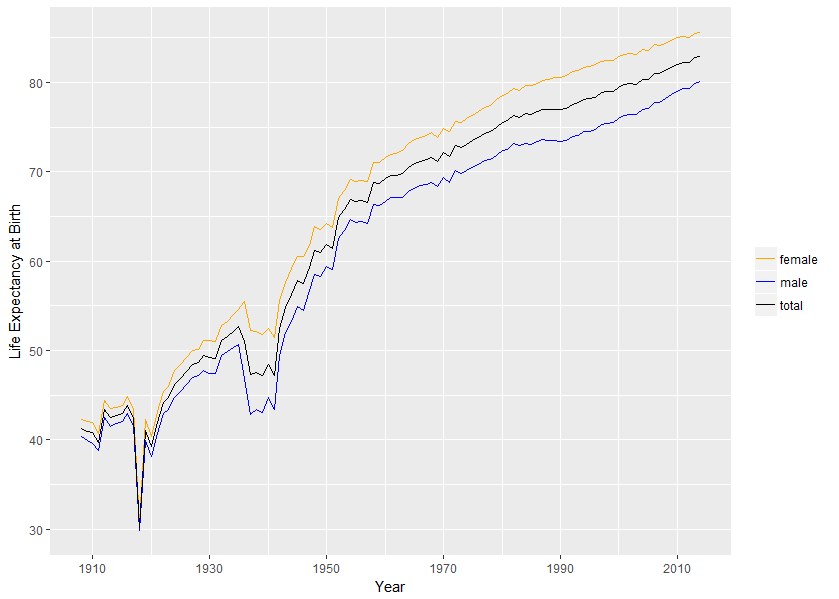
\includegraphics[width=0.7\linewidth]{LE_devel_ESP}
	\caption{Life Expectancy at Birth by Sex - Spain}
	\label{fig:ledevelesp}
\end{figure}

	%%% ------------------------------------------------ %%%
	% Bibliography %
	%%% ------------------------------------------------ %%%
\newpage
\section*{\textsf{References}}
\bibliographystyle{ieeetr}
\footnotesize{\bibliography{HHPen1}}
%http://blog.lareviewofbooks.org/essays/america-america/%
\end{document}